\multiproblem{hoop}{Consider a particle of mass $m$ as shown below.
          \begin{center}
        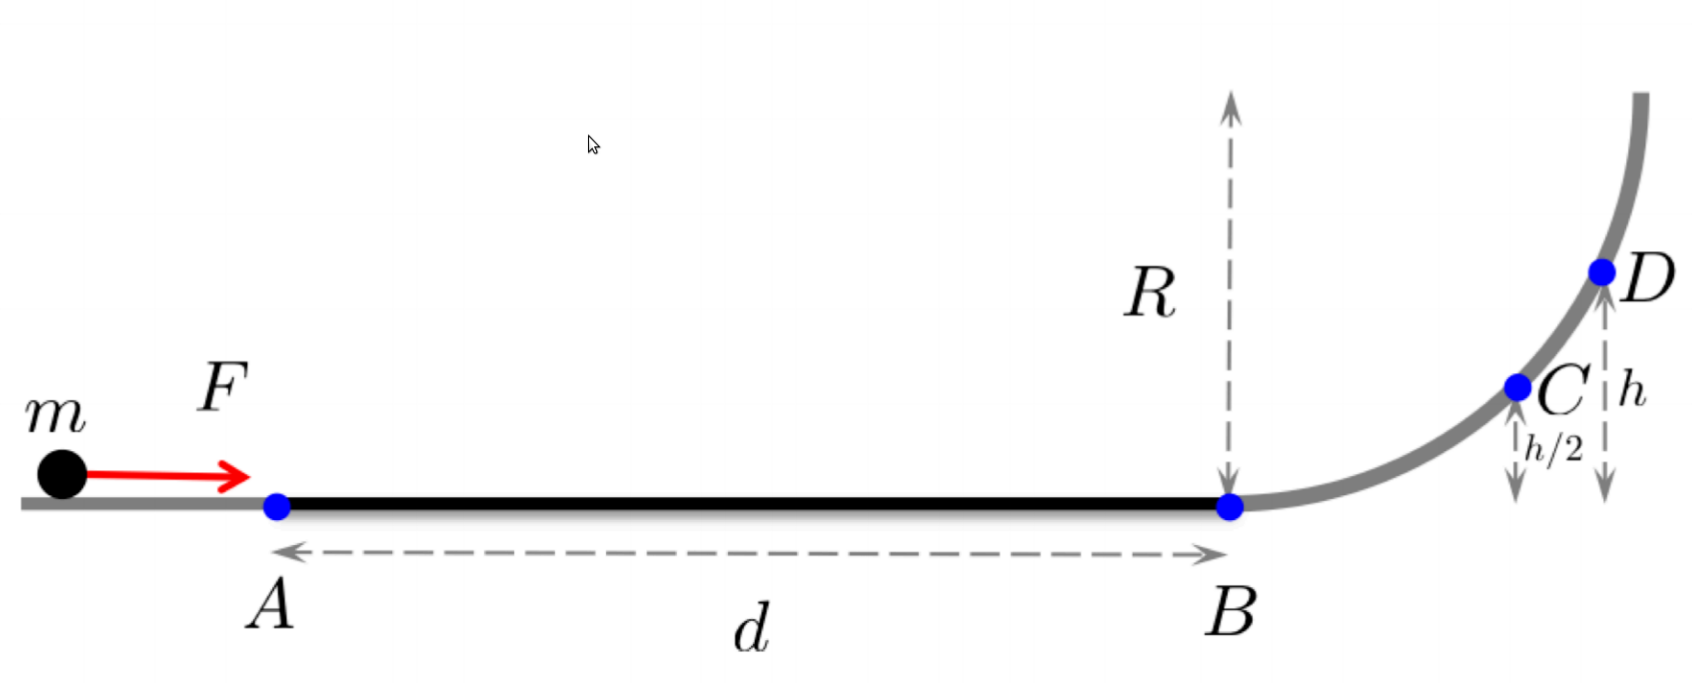
\includegraphics[width=0.5\textwidth]{hoop.pdf}
        \end{center} 
  
\begin{enumerate}
\item A constant force $F$ is applied to the particle between time $t=0$ to time $t=t_{A}$. Use the Impulse Momentum Theorem to find the velocity at time $t_{A}$, written $v_{A}:=v(t_{A})$.
\item After this, the particle moves a distance $d$ from point $A$ to point $B$, where it is subject to a frictional force proportional to its velocity $f=-\beta v$. Using Newton's 2nd Law, write an ODE (ordinary differential equation) for the velocity of the particle during this motion.
\item By using separation of variables, solve the IVP (initial value problem) made up of the ODE you have found in (b) together with the initial condition in part (a). Show that the solution, for the velocity of the particle as a function of time, is given by $v(t)=v_{A}\text{e}^{-\beta(t-t_{A})/m}$.
\item Integrate $v(t)$ with respect to time to find the position $r(t)$. (Hint: setting $r(t_{A})=0$, $r(t)=\int_{t_{A}}^{t} v(\tau) d\tau=\dots$).
\item Using the results of (c) and (d), find an equation for the velocity of the particle as a function of the position $v(r)$.
\item Find the work done on the particle from $A$ to $B$ (Hint: use your equation for $v(r)$).
\item Using the Work-Energy Theorem, find the velocity of the particle at $B$.
\item At point $B$ the particle enters a vertical frictionless hoop of radius $R$, and reaches the maximum height $h$ at point $D$. Using the conservation of total energy, calculate the velocity of the particle at point $C$.
\item The force ${\bf F}$ at point $C$ can be written in terms of its components in the directions ${\bf e}_{r}$ and ${\bf e}_{\theta}$ as ${\bf F}=F_{r}{\bf e}_{r}+ F_\theta{\bf e}_{\theta}$ respectively. Draw a free body diagram for the particle at this point. Write down Newton's 2nd Law in terms of $F_{r}$ and $F_\theta$ along each of these directions.
\item The acceleration in plane polar coordinates is given by ${\bf a}=a_{r}{\bf e}_{r}+a_{\theta}{\bf e}_{\theta} =(\ddot{r}-r\dot\theta^{2}){\bf e}_{r}+(r\ddot\theta+2\dot{r}\dot{\theta}){\bf e}_{\theta}$. What is the acceleration when the motion is circular with $r(t)=R$? Use the equation for the angular speed $\omega$ to find the relationship between radial acceleration ($a_{r}$) and speed ($v$) in a circular motion.
\item Using your result from (j) find the normal reaction of the hoop ($N$) at point $C$ as a function of $d,\beta,m,g,h$.
\end{enumerate}
}